\section{Results}\label{sec:results}
We quantify the Jao Gap location along the magnitude (Table
\ref{tab:GapLocation}) axis by sub-sampling our synthetic populations, finding
the linear number density along the magnitude axis of each sub-sample,
averaging these linear number densities, and extracting any peaks above a
prominence threshold of 0.1 as potential magnitudes of the Jao Gap (Figure
\ref{fig:JaoGapLocator}). Gap widths are measured at 50\% the height of the peak
prominence. We use the python package \texttt{scipy} \citep{2020SciPy-NMeth} to
both identify peaks and measure their widths. 

\begin{figure*}[ht!]
	\centering
	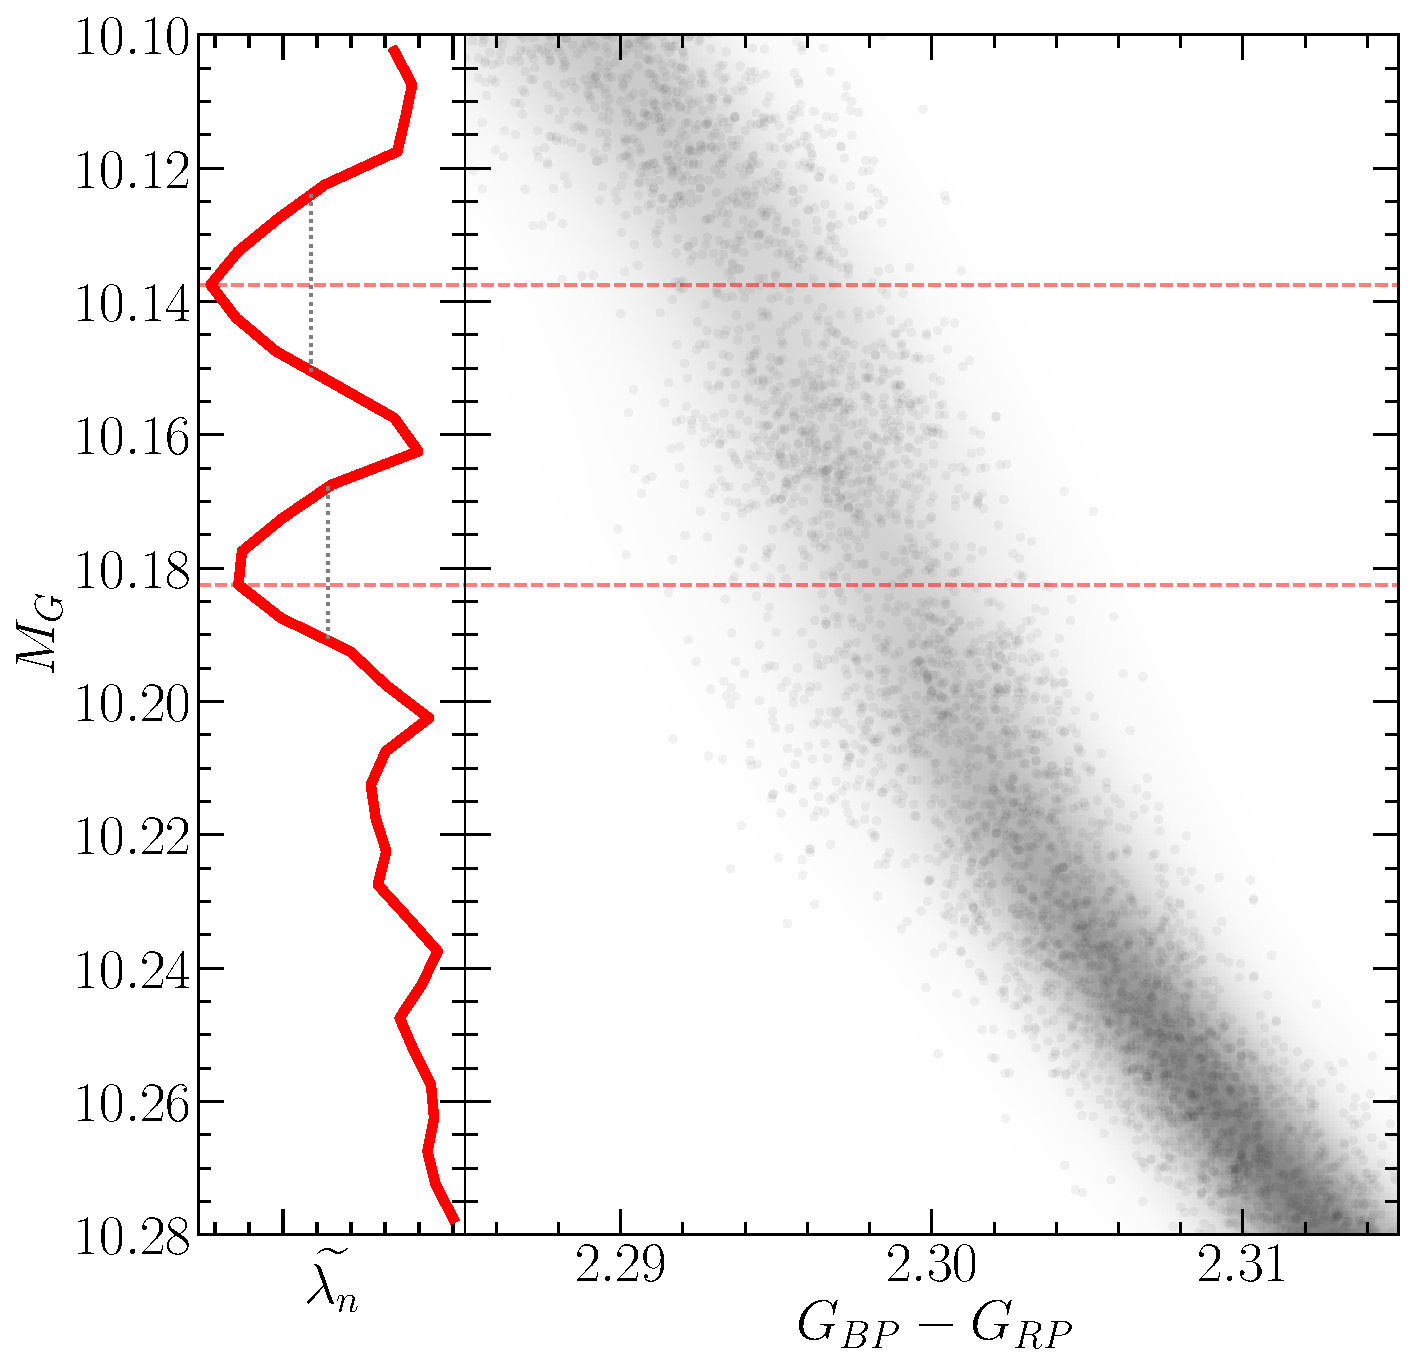
\includegraphics[width=0.45\textwidth]{OPAL_Jao_locator.pdf}
	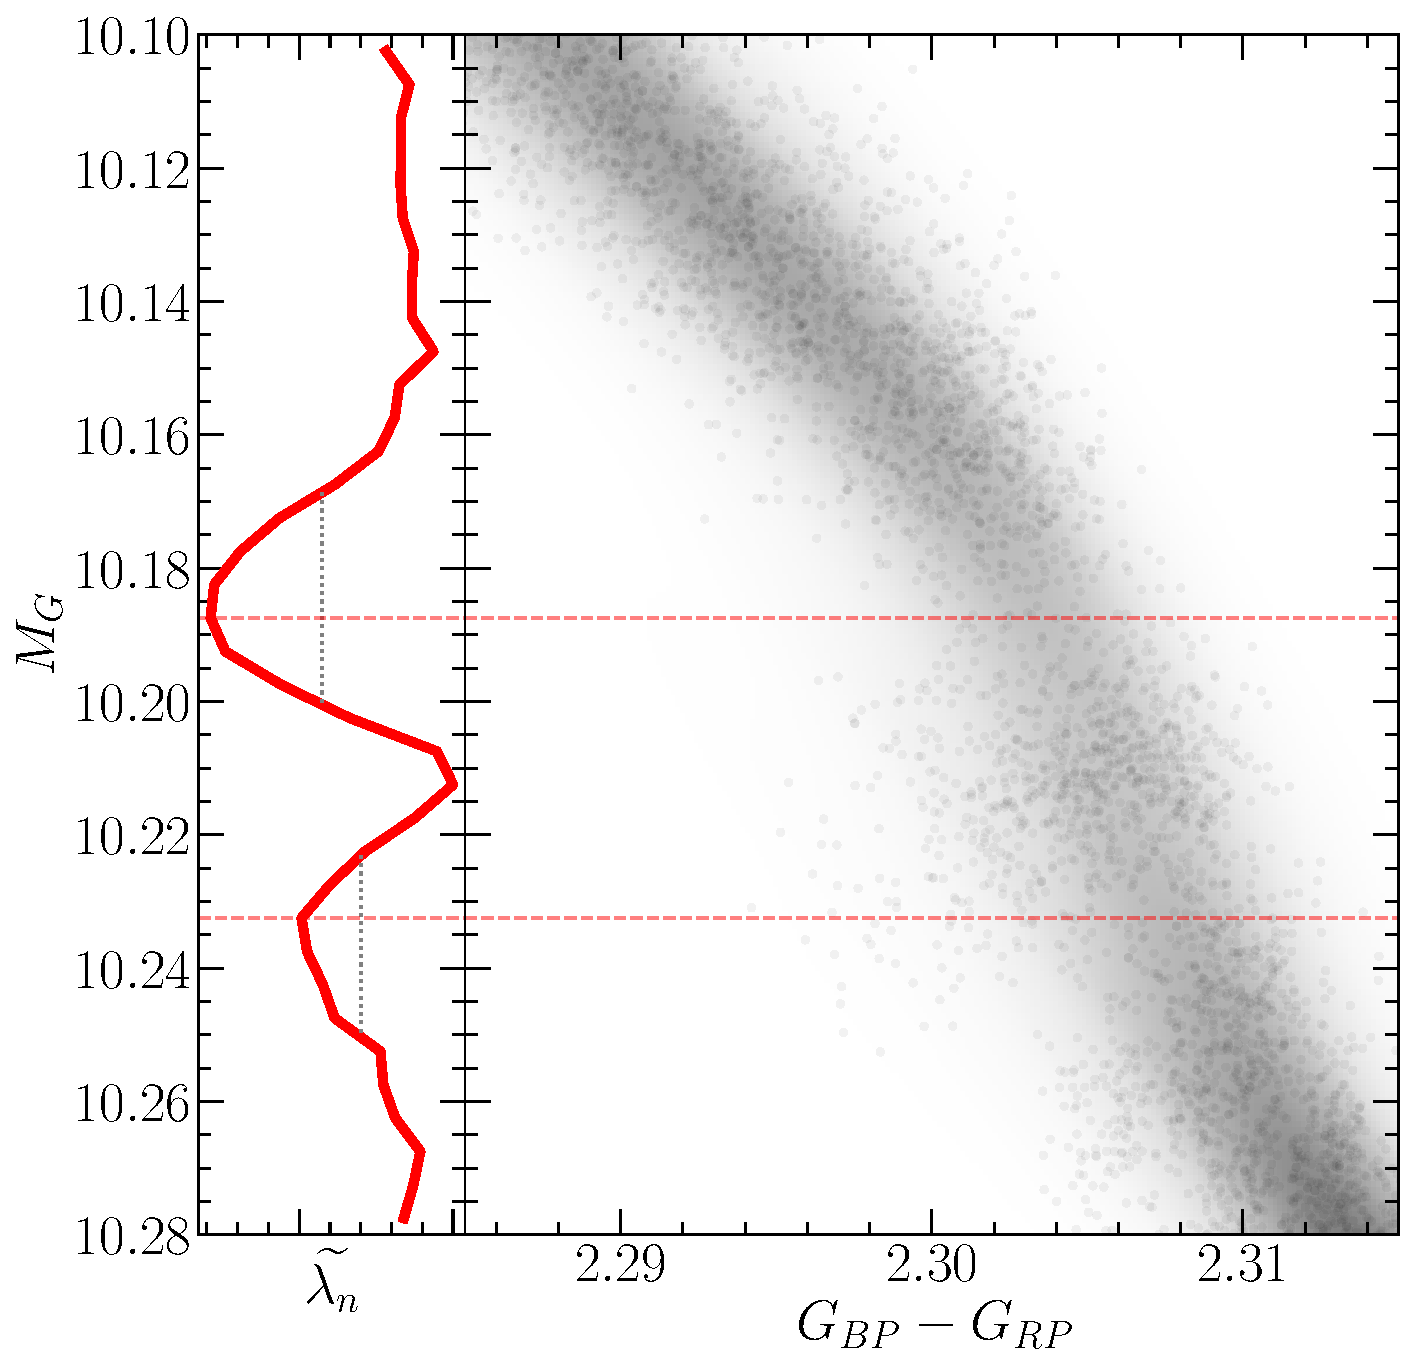
\includegraphics[width=0.45\textwidth]{OPLIB_Jao_locator.pdf}
	\caption{(right panels) OPAL (left) and OPLIB (right) synthetic
	populations. (left panels) Normalized linear number density along the
	magnitude axis. A dashed line has been extended from the peak through both
	panels to make clear where the identified Jao Gap location is wrt. to the
	population. }
	\label{fig:JaoGapLocator}
\end{figure*}

\begin{table}
	\centering
	\begin{tabular}{c | c c c}
		\hline
		Model & Location & Prominence & Width\\
		\hline
		\hline
		OPAL 1 & 10.138 & 0.593 & 0.027 \\
		OPAL 2 & 10.183 & 0.529 & 0.023 \\
		OPLIB 1 & 10.188 & 0.724 & 0.032 \\
		OPLIB 2 & 10.233 & 0.386 & 0.027 
	\end{tabular}
	\caption{Locations identified as potential Gaps.}
	\label{tab:GapLocation}
\end{table}

In both OPAL and OPLIB synthetic populations our Gap identification method
finds two gaps above the prominence threshold. The identification of more than
one gap is not inconsistent with the mass-luminosity relation seen in the grids
we evolve. As noise is injected into a synthetic population smaller features will
be smeared out while larger ones will tend to persist. The mass-luminosity
relations shown in in Figure \ref{fig:PunchIn} make it clear that there are: (1),
multiple gaps due to stars of different masses undergoing convective mixing
events at different ages, and (2), the gaps decrease in width moving to lower
masses / redder. Therefore, the multiple gaps we identify are attributable to
the two bluest gaps being wide enough to not smear out with noise. In fact, if
we lower the prominence threshold just slightly from 0.1 to 0.09 we detect a
third gap in both the OPAL and OPLIB datasets where one would be expected.

Previous modeling efforts \citep[e.g.][]{Feiden2021} have not identified
multiple gaps. This is likely due to two reasons: (1), previous studies have
allowed metallicity to vary across their model grids, further smearing the gaps
out, and (2), previous studies have used more coarse underlying mass grids,
obscuring features smaller than their mass step. While this dual-gap structure
has not been seen in models before, a more complex gap structure is not totally
unprecedented as \citet{Jao2021} identifies an additional under-dense region
below the primary gap in EDR3 data. As part of a follow up series of papers, we
are conducting further work to incorporate metallicity variations while still
using the finer mass sampling presented here.


The mean gap location of the OPLIB population is at a fainter magnitude than
the mean gap location of the OPAL population. Consequently, in the OPLIB sample
the convective mixing events which drive the kissing instability begin
happening at lower masses (i.e. the convective transition mass decreases). A
lower mass range will naturally result in a fainter mean gap magnitude.

\begin{figure}
	\centering
	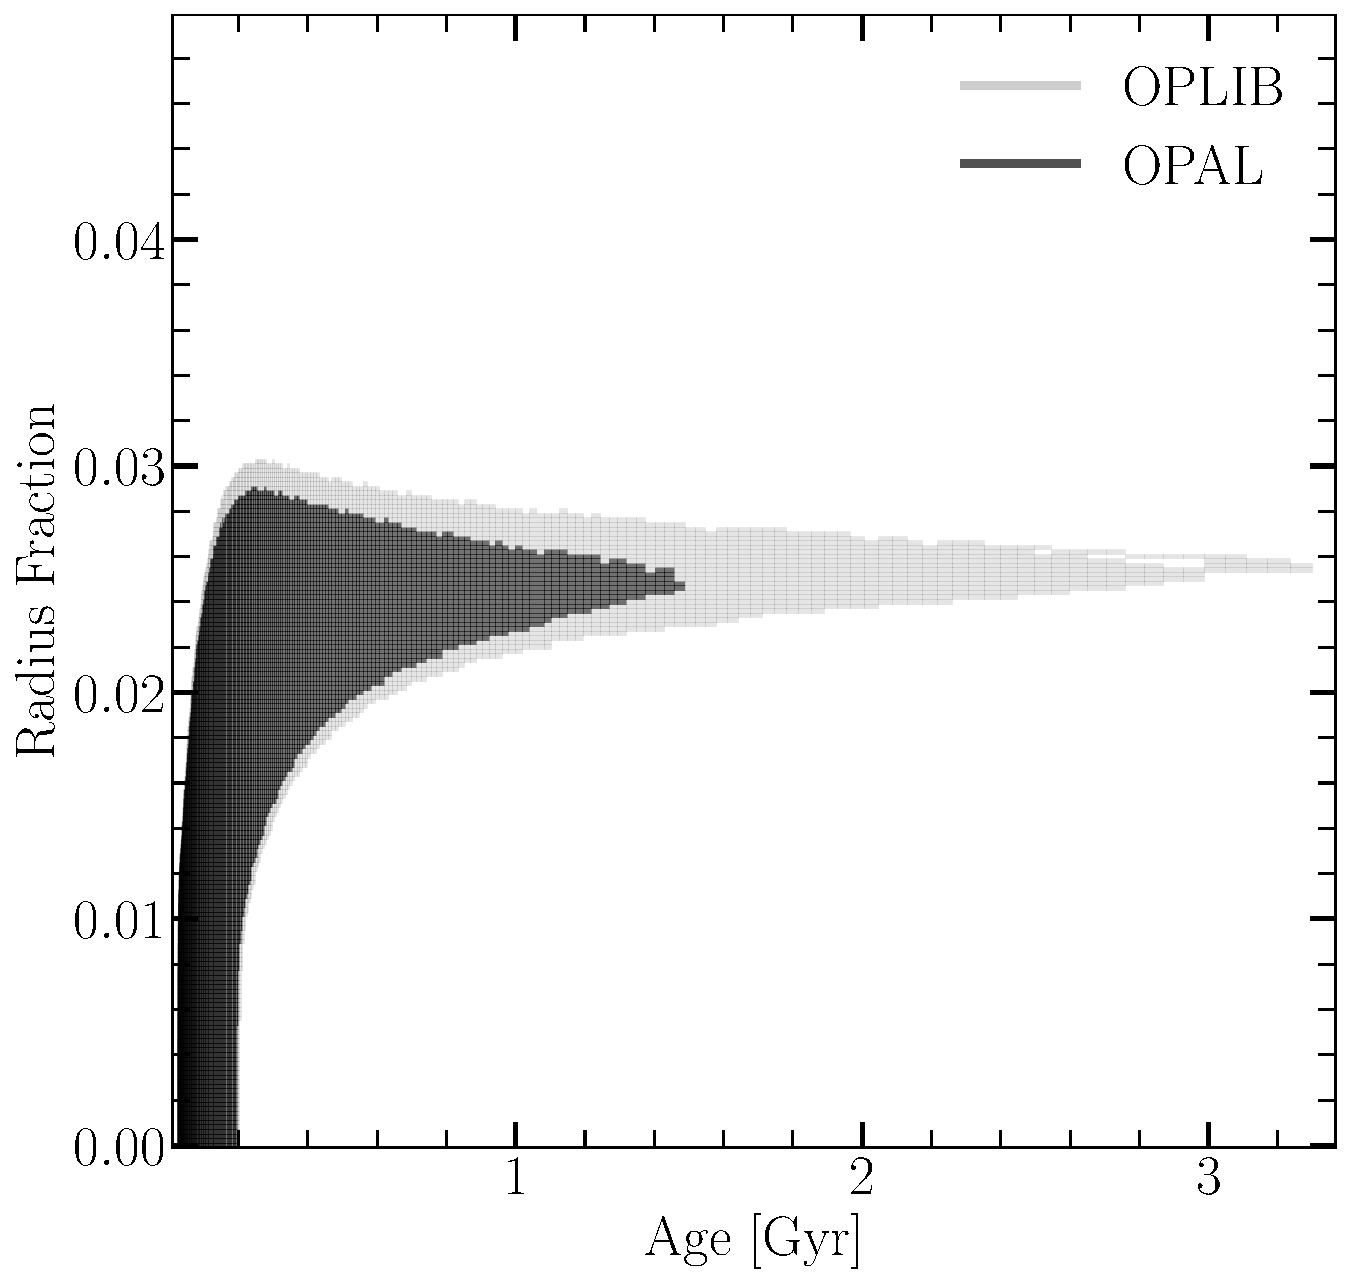
\includegraphics[width=0.45\textwidth]{SameMassConvectiveZoneComp.pdf}
	\caption{Portions of 0.3526 $M_{\odot}$ OPAL and OPLIB stellar models
	showing the interior shells which are radiative (black region). Note that
	for clarity only one convective mixing event from each model is shown. Note
	how the radiative zone in the OPLIB model is larger.}
	\label{fig:Unstable}
\end{figure}

Mixing events at lower masses in OPLIB models are attributable to the radially
thicker, at the same mass, radiative zones (Figure \ref{fig:Unstable}). This
thicker radiative zone will take more time to break down and is characteristic
of OPLIB models as of a result of their slightly lower opacities. A lower
opacity fluid will have a more shallow radiative temperature gradient than a
higher opacity fluid; however, as the adiabatic temperature gradient remains
essentially unchanged as a function of radius, a larger interior radius of the
model will remain unstable to radiation. This thicker radiative zone will
increase the time it takes the core convective zone to meet up with convective
envelope meaning that lower mass models can sustain a radiative zone for
longer than they could otherwise; thus; lower opacities push the convective
transition mass down. We can additionally see this longer lived radiative zone
in the core $^{3}$He mass fraction, in which OPLIB models reach much higher
concentrations --- at approximately the same growth rate --- for the same mass
as OPAL models do (Figure \ref{fig:OPALOPLIB3He}). 

The most precise published Gap location comes from \citet{Jao2020} who use EDR3
to locate the Gap at $M_{G} \sim 10.3$, we identify the Gap at a similar
location in the GCNS data. The Gap in populations evolved using OPLIB
tables is closer to this measurement than it is in populations evolved using
OPAL tables (Table \ref{tab:GapLocation}). It should be noted that the exact
location of the observed Gap is poorly captured by a single value as the Gap
visibly compresses across the width of the main-sequence, wider on the blue
edge and narrower on the red edge such that the observed Gap has downward
facing a wedge shape (Figure \ref{fig:JaoGap}). This wedge shape is not
successfully reproduced by either any current models or the modeling we preform
here. We elect then to specify the Gap location where this wedge is at its
narrowest, on the red edge of the main sequence.

\begin{figure}
	\centering
	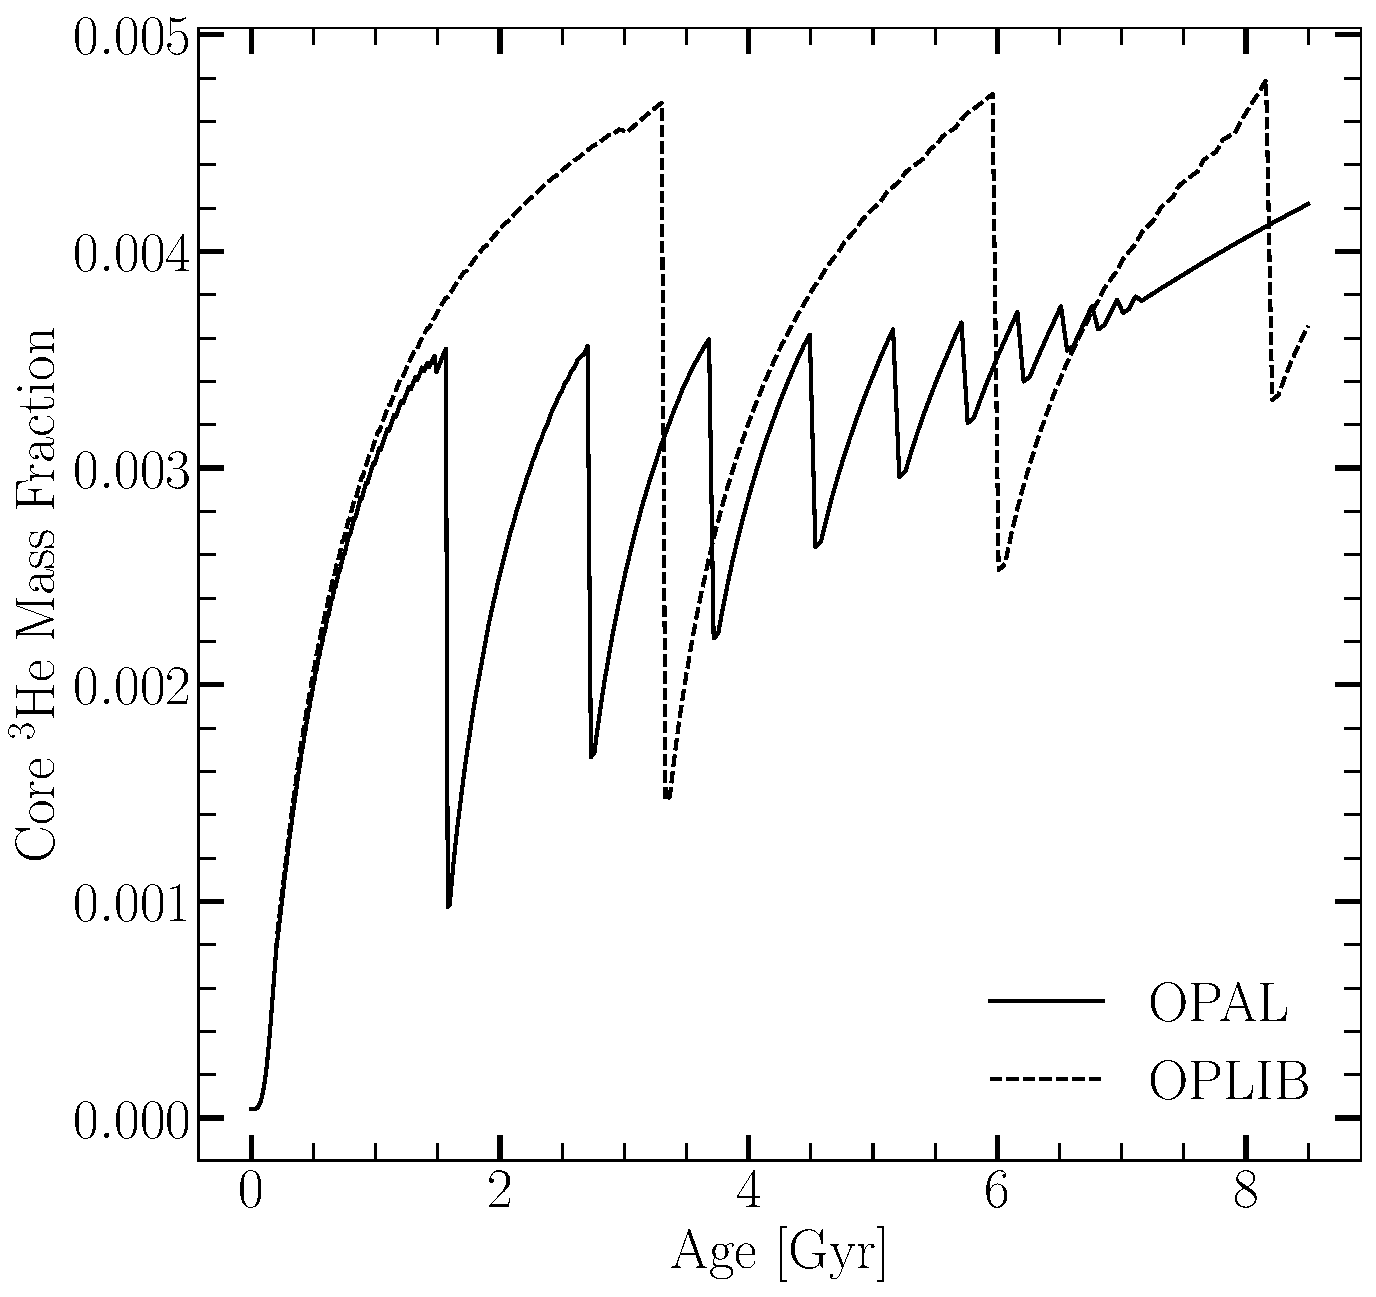
\includegraphics[width=0.45\textwidth]{Core3HECompSameMass.pdf}
	\caption{Core $^{3}$He mass fraction for  0.3526 $M_{\odot}$ models evolved
	with OPAL and OPLIB (within the Jao Gap's mass range for both). Note how
	the OPLIB model's core $^{3}$He mass fraction grows at approximately the
	same rate as the OPAL model's but continues uninterrupted for longer.}
	\label{fig:OPALOPLIB3He}
\end{figure}

The Gaps identified in our modeling have widths of approximately 0.03
magnitudes, while the shift from OPAL to OPLIB opacities is 0.05 magnitudes.
With the prior that the Gaps clearly shift before noise is injected we know
that this shift is real. However, the shift magnitude and Gap width are of
approximately the same size in our synthetic populations. Moreover,
\citet{Feiden2021} identify that the shift in the modeled Gap mass from [Fe/H]
= 0 to [Fe/H] = +0.5 as 0.04$M_{\odot}$, whereas we only see an approximate
$0.01$ M$_{\odot}$ shift between OPAL and OPLIB models. Therefore, the
Gap location will likely not provide a usable constraint on the opacity
source.
